\chapter{Introduction}\label{introduction}

\ifpdf
    \graphicspath{{Chapter1/Figs/Raster/}{Chapter1/Figs/PDF/}{Chapter1/Figs/}}
\else
    \graphicspath{{Chapter1/Figs/Vector/}{Chapter1/Figs/}}
\fi


\section{Motivation}

\NOTE{D}{Also, balls into bins is an established framework for load balancing and hashing. You should not need too much text. (e.g. refer to the survey by Wieder and perhaps Cuckoo hashing)}

Load balancing has been an important topic for many years, and it has gained even more attention recently (e.g.\ cloud computing~\cite{mishra2020cloud} \NOTE{T}{Not a very good reference. Instead you should use the Wieder survey for example. Andor: I use that a few paragraphs later when I say it is more than just load balancing. Here I wanted to highlight that it gained more attention recently with new areas such as cloud computing. Is it not a good idea?}). In the usual setup, there are some servers, and whenever a job arrives, the goal is to allocate it to one of the servers such that no server is overloaded (which at high burden often requires also that no server is underloaded). At first glance, it might seem an easy problem to solve: always allocate the job greedily to the currently least loaded server. Or even simpler, in the case of homogeneous jobs: apply round-robin scheduling to the servers, using each of them in a cyclic way. 

The problem with these approaches is that they require a centralised load balancer. That central\NOTE{D}{This} load balancer would be\NOTE{D}{is} a single point of failure, reducing the robustness of the whole\NOTE{D}{remove whole?} system, and decreasing performance due to its sequential nature (e.g. \NOTE{D}{not all Google search requests can...}all Google search requests cannot go through a single machine). An alternative is to use \NOTE{D}{distributed ?}randomised load balancing. The idea is to allocate the jobs according to a random protocol -- the simplest being choosing a server uniformly at random -- that can be run independently on each client (requesting the job), without a central load balancer. The obvious question\NOTE{D}{key challenge} is how to shape\NOTE{D}{design} this random protocol such that a good balance is achieved. A groundbreaking result in this topic was presented in~\cite{azar1999twochoice}. They showed that the \TwoChoice protocol, which always\NOTE{D}{Remove always} randomly queries the load of two independent servers, and allocates the job into the lesser loaded of the two, achieves a maximum load of $\frac{\ln(\ln(n))}{\ln(2)} + O(1)$ with $n$ servers after $n$ jobs, with high probability (meaning that as $n$ goes to infinity, the probability converges to $1$). This result led to extensive further study of the topic (see e.g.~\cite{richa2001surveytwochoice}), and even\NOTE{D}{several} large companies, such as Twitter started using this idea (often called ``The power of Two-Choices'')~\cite{anderson2019twitter}.


There are various versions of the load balancing problem (e.g.\ homogeneity of the jobs, random protocol used\NOTE{D}{The setting does not depend on the choice of protocol. Maybe just say ``There are several versions of the load balancing problem, making different assumptions about the jobs and the servers.''?}), and so for consistency reasons, most of the research community adapted\NOTE{D}{This part does not read clearly} the following standard abstraction: the servers are bins, and the jobs are \NOTE{D}{unit weight ?}balls. This is what I will use in the later chapters as well. This has the further advantage, that random protocols such as \TwoChoice have proved to be useful outside the field of load balancing too, e.g.\ hashing~\cite{azar1999twochoice} -- see~\cite{wieder2017ballsintobinslandscape} for a comprehensive survey. I will provide a more rigorous\NOTE{D}{``more rigorous'' to ``formal''} definition of the balls-into-bins abstraction in Chapter~\ref{preparation}.
\NOTE{D}{By presenting the gap bounds in the case $m = n$, you don't show the major benefit of \TwoThinning over \OneChoice}

There are other random protocols suggested, that \NOTE{D}{under some circumstances (and remove from the end)}are more realistic, or more efficient than \TwoChoice in some circumstances. For example, we can see that\NOTE{D}{remove ``we can see that''} if both of the bins queried by \TwoChoice have very low load, then,\NOTE{D}{remove comma} it was unnecessary to query both (e.g.\ communication overhead, slows down servers), and only one of them would be enough. \OneChoice, however, which simply allocates the ball uniformly at random (``takes 1\NOTE{D}{one} sample and accepts that'') has been shown to have an exponentially worse maximum load of $(1+o(1))\cdot \frac{\ln(n)}{\ln(\ln(n))}$ (see e.g.\ the Randomised Algorithms course\NOTE{D}{Cite ``Balls into Bins'' - A Simple and Tight Analysis (1998) OR ``Probability and Computing'' }), so it is often not sufficient. \NOTE{D}{New paragraph}Something in the middle\NOTE{D}{A process in-between \OneChoice and \TwoChoice is} is \TwoThinning~\cite{feldheim2021thinning}, which samples one bin (\NOTE{D}{the}``primary bin''), and either accepts that, or concludes that its load is too high, in which case the ball is allocated uniformly at random into one of the bins (see Figure~\ref{two-thinning-intro}). This, on average,\NOTE{D}{On average, \TwoThinning} requires less than $2$ queries per ball, but it \NOTE{D}{also}requires a decision strategy (or just ``strategy'') for whether to accept or reject a bin. This dissertation is about optimising such strategies in protocols like \TwoThinning, which I will call ``parametric protocols'' as they all require some extra ``parameter'', usually a decision strategy. The goal is to optimise some objective function measuring how ``balanced'' the load distribution is, such as the maximum load of the bins after some number of balls have been allocated.



\begin{figure}
    \centering
    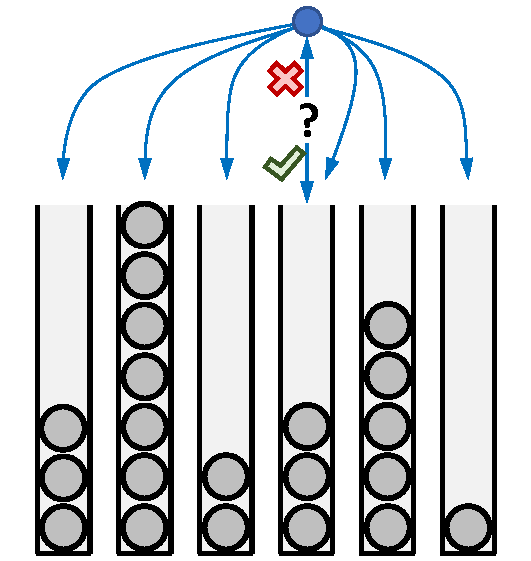
\includegraphics{Chapter1/Figs/two_thinning_intro.pdf}
    \caption{One step of the \TwoThinning protocol. The fourth bin was chosen uniformly at random, so the strategy has to decide whether to place the ball there or into a bin chosen uniformly at random. \NOTE{A}{Should I explain it here as well?}}
    \label{two-thinning-intro}
\end{figure}


\NOTE{D}{A figure with \TwoThinning would be quite useful here.}

\section{My approach}

For finding good strategies, I will compare Reinforcement Learning (RL) methods with more classical approaches (e.g.\ dynamic programming) and other heuristics (e.g.\ mean thinning). RL is a natural choice, since we have to make optimal decisions (``choose optimal thresholds for accept/reject'') in a dynamic, stochastic process. RL \NOTE{D}{Maybe: adjusts the strategy by collecting rewards. There are several options for when the reward is collected?}is based on collecting rewards, and a first idea could be getting a reward only after all the balls have been allocated (end of an execution)\NOTE{D}{The text in parentheses can be removed}, based on the final load distribution. There is more refinement needed, however, to make it work properly, which I will discuss in later chapters.\NOTE{D}{More details in Section ?? and ??} RL has already been applied to load balancing in the literature\NOTE{D}{Remove ``in the literature''}, mostly related to networking~\cite{attiah2020RLcellular, yeo2021controller}, but they\NOTE{D}{the setting is considerably different from balls-into-bins?} use an abstraction slightly different from the balls-into-bins mode. The parametric balls-into-bins protocols I will study received much attention in the academic community only recently, though there have been earlier, mostly empirical studies as well (see. e.g.~\cite{derek1986twothinningfirstattempt}).\NOTE{D}{\textsc{Thinning} has been known for quite some time in applied load balancing~\cite{derek1986twothinningfirstattempt}, but only recently some instances of these protocols were analysed~\cite{feldheim2021longtermthinning,los2022cachingpackingthinningtwinning}} At the moment, there are strategies (e.g.\ for \TwoThinning) that are proven to be asymptotically optimal, i.e., the achieved gap is optimal up to constant factors (for sufficiently large $n$). Therefore, these results are of less help directly in real-world scenarios, where there are much less number of jobs and servers. There are three reasons why most of these theoretical results are not applicable for small values: 1) \NOTE{D}{results may only hold for ``sufficiently large'' values of balls and bins.}the inequalities in the proofs do not work for small values~\cite{feldheim2021longtermthinning} so the theoretical guarantees might not hold, 2) \NOTE{D}{Constant factors in big-Oh notation are large.}the constant factor overhead in the result is significant and 3) suggested \textit{positive} integer parameter values used by the strategy would equal to $0$, e.g.\ $\floor{\ln(\ln(\ln(\mathrm{number\ of\ servers})))}$ which is usually $0$ even for large datacenters~\cite{uzaman2019datacentersize}.

\NOTE{D}{Maybe start with the description of the protocol. ``An alternative implementation of \TwoThinning is: 1) .... . This is more natural and effective because ....}Looking at the practical application of the \TwoThinning protocol, it is often much more natural and effective if the queried server itself decides whether to take the job, rather than sending back its current load value back to the client which makes the decision whether to accept of reject that server.  Overall, the process is 1) the client chooses a server uniformly at random, 2) the server either completes the job or passes it on to a server chosen uniformly at random.

The important question left is what information can the server use in deciding whether to accept a job or not. It needs some ``reference'' to assess its load relative to others, which requires some centralised information. There are several options, for example the servers could maintain the total number of jobs in the system, or they could synchronise their individual loads from time-to-time (see e.g.~\cite{zhang2018datacenterloadbalancing} for efficient communication in data centers). I will focus on the latter, which crucially allows a server to make its decision based on the (possibly slightly outdated) loads of all the other servers. When a server decides to pass on the job to another one, the motivation for choosing the other server at random is that due to parallelism and the possibly outdated information, the seemingly least loaded server could quickly become the most overloaded if all the other servers pass the jobs to that one.


Having introduced the practical details, I will take a more theoretical approach in this project. Realising the lack of exact, non-asymptotical results even for simple protocols, and to simplify the analysis, I will try to solve a simpler problem than the practical one presented above: the strategy is given the \textbf{exact load distribution} at the moment, and it is offered a specific (``primary'') bin, which it can either accept and place the ball there, or reject, in which case the ball is allocated to a ``secondary'' bin chosen uniformly at random. Another big simplification is that all the balls are allocated by a single instance of the strategy sequentially, i.e.\ the load distribution depends only on its own allocations. We will see that finding a good strategy even for this greatly simplified version proves to be very challenging for RL and other algorithms. When describing the candidate strategies I will highlight those that are more directly applicable in more realistic scenarios. \NOTE{A}{This is the single most important paragraph in the dissertation! Check if it is 100\% clear to the reader, both the motivation and the simplified problem.}


Overall, the intention of this dissertation is more to survey the applicability of RL and other approaches in different protocols, than to provide directly practical protocols. Another aim of the project is to gain a deeper insight to how an optimal strategy looks like.


\NOTE{D}{As discussed in the last meeting, even the non-RL setting you give it a load distribution and the NN needs to pick a threshold that will be used for the next $K$ steps is interesting, because it could work in a batched setting. Andor: what should I do with it?}


\section{Outline}

The outline of the dissertation is as follows.


In Chapter~\ref{preparation}, I define the balls-into-bins terminology and its assumptions more precisely\NOTE{D}{I formally define the balls-into-bins setting, its terminology and the core protocols.}, describing the balls-into-bins protocols that I will analyse in later chapters -- I do not discuss all of them at such length as I did in this chapter for \TwoThinning, but similar practical considerations apply\NOTE{A}{Is this sentence needed?}\NOTE{D}{No, remove}. Finally, I explain the basics of RL, with particular focus on \DQL, which is the main algorithm that I used.


In Chapter~\ref{implementation}, I explain the implementation details of the RL algorithms and other strategies (such as dynamic programming)\NOTE{D}{Dynamic programming is one of the main implementation milestones, so maybe list it at the same level as RL.}, for various parametric protocols, highlighting several improvements implemented for speedup and better performance\NOTE{D}{The last part does not read well}.


In Chapter~\ref{evaluation}, I compare the implemented approaches from different\NOTE{D}{various} aspects, including how well they can balance the load, their training complexity (if any) and their behaviour. I also provide several insights via a thorough hyperparameter analysis for RL, and as an extension, lemmas and conjectures about optimal strategies.

In Chapter~\ref{conclusion}, I conclude with some future work ideas for improving the RL approaches, gaining better insights to optimal strategies, and extending the study to different protocols.